% Number 951
% CAPMG Units 
% Car slowing, a given - graphical
% JG

% Watermark
\AddToShipoutPicture*{\BackgroundPic}

\addtocounter {ProbNum} {1}

%\begin{floatingfigure}[r]{.44\textwidth}
%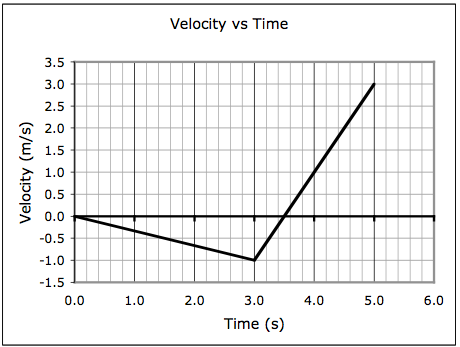
\includegraphics[scale=.54]{/Users/jgates/desktop/latex/pics/vgraph6}
%\end{floatingfigure}
 
{\bf \Large{\arabic{ProbNum}}} A car drives down the road at ${18~\tfrac{m}{s}}$.  It slows down at a rate of ${2.2~\tfrac{m}{s}}$ per second.  \bigskip

After how much time will it be moving with a speed of ${7~\tfrac{m}{s}}$? Use graphical methods.
\vfill

How far did the car travel during the motion described above? Use graphical methods.
 \vfill


%\begin{center}
%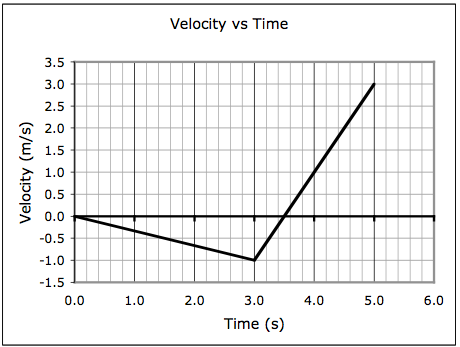
\includegraphics[scale=1]{/Users/jgates/desktop/latex/pics/vgraph6}
%\end{center}


\newpage